\documentclass[border=.2cm]{standalone}
\usepackage{tikz}
\usepackage{amsmath}

\begin{document}

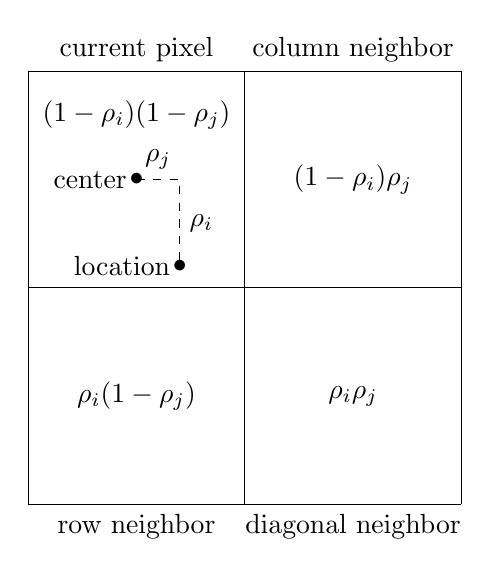
\begin{tikzpicture}
    \def \length {5.5};
    \foreach \ii in {0, \length*.5, \length} {
        \draw (\ii, 0) --++ (0, \length);
        \draw (0, \ii) --++ (\length, 0);
    }
    \node[above] at (0.25*\length, \length) {current pixel};
    \node[above] at (0.75*\length, \length) {column neighbor};
    \node[below] at (0.25*\length, 0) {row neighbor};
    \node[below] at (0.75*\length, 0) {diagonal neighbor};
    \draw[dashed] (.25*\length,.75*\length) coordinate(O) node {$\bullet$} node[left] {center} --++ (0.1*\length, 0) node[midway, above] {$\rho_j$} --++ (0,-.2*\length) node[midway, right] {$\rho_i$} node {$\bullet$} node[left] {location};
    \node at (.25*\length, .9*\length) {$(1-\rho_i)(1-\rho_j)$};
    \node at (.75*\length, .75*\length) {$(1-\rho_i)\rho_j$};
    \node at (.25*\length, .25*\length) {$\rho_i(1-\rho_j)$};
    \node at (.75*\length, .25*\length) {$\rho_i\rho_j$};
\end{tikzpicture}

\end{document}